\documentclass[prd,amssymb,amsmath,amsfonts,nofootinbib,reprint,showpacs,longbibliography]{revtex4-1}

\usepackage{graphicx}
\usepackage{lmodern}
\usepackage{amsmath,amssymb}
\usepackage{mathrsfs}
\usepackage{amsfonts}
\usepackage[utf8]{inputenc}
\usepackage{url}
\usepackage[colorlinks]{hyperref}
\usepackage[table]{xcolor}
\usepackage{multirow}
\usepackage[normalem]{ulem}
\usepackage{lipsum}

\usepackage{marvosym}
\usepackage{enumerate}
\usepackage{color,soul}
\usepackage{acronym}

\usepackage{bm}
\usepackage{color}
\usepackage{commath}
\allowdisplaybreaks
\usepackage{multirow}

\def\lm{{\ell m}}
\newcommand{\avg}[1]{\rangle{#1}\langle}
\newcommand{\scri}{{\mathrsfs{I}}}
\newcommand{\stf}[1]{{\langle {#1} \rangle}}
\newcommand{\ord}{\mathcal{O}}
\newcommand{\f}{\frac}
\newcommand{\gsf}{\text{1GSF}}
\newcommand{\bk}{\text{0GSF}}
\newcommand{\el}{\ell}
\newcommand{\nn}{\nonumber}
\newcommand{\mbf}[1]{\mathbf{#1}}
\newcommand{\LOhat}{\!\hat{\,\mathbf{L}}_0}
\newcommand{\Lhat}{\!\hat{\,\mathbf{L}}_\text{N}}
\newcommand{\Jhat}{\hat{\mathbf{J}}_\text{N}}
\newcommand{\Sa}{\mbf{S}_1}
\newcommand{\Sb}{\mbf{S}_2}
\newcommand{\hs}{\hat{s}}
\newcommand{\hS}{\hat{S}}
\newcommand{\Lhatdot}{\dot{\hat{\,\mathbf{L}}}_\text{N}}
\newcommand{\LhatdotNew}{\dot{\hat{\,\mathbf{L}}}_{\text{N},\perp}}
\newcommand{\Sadot}{\dot{\mbf{S}}_1}
\newcommand{\Sbdot}{\dot{\mbf{S}}_2}
\newcommand{\Jdot}{\dot{\mbf{J}}}
\newcommand{\rdot}{\dot{\mbf{r}}}
\newcommand{\vdot}{\dot{\mbf{v}}}
\newcommand{\ud}{\mathrm{d}}
\newcommand{\Ldot}{\dot{\mbf{L}}_{\text N}}
\newcommand{\LN}{\mbf{L}_{\text N}}
\newcommand{\nnm}{\nonumber}
\newcommand{\mce}{\mathcal{E}}
\newcommand{\mcb}{\mathcal{B}}

\def\TEOBResumS{\texttt{TEOBResumS}}
\def\TEOBResumSGIOTTO{\texttt{TEOBResumSGIOTTO}}
\def\TEOBResumSecce{\texttt{TEOBResumSecce}}
\def\bajes{\texttt{bajes}}
\def\Boldtheta{\boldsymbol{\theta}}
\def\Boldd{\textbf{d}}
\def\TEOBResumSDali{\texttt{TEOBResumS-Dalí}}
\def\TEOBB{\texttt{Beyond-TEOBResumS}}
\def\c3{c_{\rm{N}^3\rm{LO}}}
\def\mbhf{M_{\rm BH}^f}
\def\abhf{a_{\rm BH}^f}
\def\alphalm0{\alpha_{\ell m 0}}
\def\taulm0{\tau_{\ell m 0}}
\def\omegalm0{\omega_{\ell m 0}}


% Define capitalized acronyms
\newacro{adm}[ADM]{Arnowitt-Deser-Misner}
\newacro{bbh}[BBH]{binary black hole}
% \newacroplural{bbh}[BBHs]{binary black holes}
\newacro{bh}[BH]{black hole}
\newacroplural{bh}[BHs]{black holes}
\newacro{bhns}[BHNS]{black hole-neutron star}
\newacro{bhpt}[BHPT]{black hole perturbation theory}
\newacro{bns}[BNS]{binary neutron star}
\newacro{bf}[BF]{Bayes' factor}
\newacro{cbc}[CBC]{compact binary coalescence}
\newacro{ce}[CE]{Cosmic Explorer}
\newacro{da}[DA]{data analysis}
\newacro{et}[ET]{Einstein Telescope}
\newacro{eob}[EOB]{Effective-One-Body}
\newacro{eom}[EOM]{equations of motion}
\newacro{fd}[FD]{frequency domain}
\newacro{fft}[FFT]{Fast Fourier transform}
\newacro{gw}[GW]{gravitational-wave}
\newacroplural{gw}[GWs]{Gravitational-waves}
\newacro{gr}[GR]{general relativity}
\newacro{grb}[GRB]{gamma-ray burst}
\newacro{grhd}[GRHD]{general-relativistic hydrodynamics}
\newacro{gwosc}[GWOSC]{Gravitational Wave Open Science Center}
\newacro{gwtc1}[GWTC-1]{the first gravitational-wave transients catalog}
\newacro{gsf}[GSF]{Gravitational Self Force}
\newacro{hm}[HM]{Higher mode}
\newacroplural{hm}[HMs]{Higher modes}
\newacro{ifo}[IFO]{interferometer}
\newacro{imr}[IMR]{inspiral-merger-ringdown}
\newacro{im}[IMR]{inspiral-to-merger}
\newacro{kagra}[KAGRA]{Kamioka Gravitational Wave Detector}
\newacro{ligo}[LIGO]{Laser Interferometer Gravitational-Wave Observatory}
\newacro{lisa}[LISA]{Laser Interferometer Space Antenna}
\newacro{lr}[LR]{Light Ring}
\newacro{lso}[LSO]{Last Stable Orbit}
\newacro{lvc}[LVC]{LIGO-Virgo Collaboration}
\newacro{lvk}[LVK]{LIGO-Virgo-Kagra Collaboration}
\newacro{lo}[LO]{leading order}
\newacro{ns}[NS]{neutron star}
\newacroplural{ns}[NSs]{neutron stars}
\newacro{nr}[NR]{numerical relativity}
\newacro{nqc}[NQC]{Next-to-quasicircular corrections}
\newacro{nlo}[NLO]{next-to-leading order}
\newacro{nnlo}[NNLO]{next-to-next-to-leading order}
\newacro{n3lo}[N3LO]{next-to-next-to-next-to-leading order}
\newacro{n4lo}[N3LO]{next-to-next-to-next-to-next-to-leading order}
\newacro{ode}[ODE]{Ordinary Differential Equation}
\newacroplural{ode}[ODEs]{Ordinary Differential Equations}
\newacro{pn}[PN]{post-Newtonian}
\newacro{pm}[PM]{post-Minkowskian}
\newacro{pe}[PE]{parameter estimation}
\newacro{psd}[PSD]{power spectral density}
\newacro{pa}[PA]{post-adiabatic}
\newacro{qnm}[QNM]{quasi-normal mode}
\newacro{qc}[QC]{quasi-circular}
\newacro{snr}[SNR]{signal-to-noise ratio}
\newacro{spa}[SPA]{stationary-phase approximation}
\newacro{sxs}[SXS]{Simulating eXtreme Spacetimes}
\newacro{td}[TD]{time domain}
\newacro{ng}[NG]{Nect Generation}


\definecolor{cyan}{rgb}{0,0.9,0.9}
\definecolor{orange}{rgb}{0.9,0.5,0}
\definecolor{magenta}{rgb}{1,0,1}
\definecolor{purple}{rgb}{0.8,0.4,0.8}
\definecolor{gray}{rgb}{0.8242,0.8242,0.8242}
\definecolor{dodgerblue}{rgb}{0.12, 0.56, 1.0}

\newcommand{\RG}[1]{{\textcolor{dodgerblue}{{RG: #1}} }}
\newcommand{\JL}[1]{{\textcolor{purple}{{JL: #1}} }}
\newcommand{\DC}[1]{{\textcolor{orange}{{DC: #1}} }}
\newcommand{\NC}[1]{{\textcolor{magenta}{{NC: #1}} }}


\newcommand{\todo}[1]{\textcolor{red}{\texttt{TODO: #1}}} 
\newcommand{\red}[1]{\textcolor{red}{#1}} 
\newcommand{\bl}[1]{\textcolor{blue}{#1}} 
\newcommand{\cor}[2]{\sout{#1}\textcolor{red}{#2}} 
\newcommand{\old}[1]{\textcolor{gray}{\sout{#1}}}
\newcommand{\new}[1]{\red{#1}}

\newcommand{\eo}[0]{\hat{E}_0}
\newcommand{\lo}[0]{\hat{L}_0}
\newcommand{\bphi}[0]{\bar{\varphi}}
\newcommand{\dbphi}[0]{\dot{\bar{\varphi}}}
\newcommand{\dphi}[0]{\dot{\varphi}}
\newcommand{\amrg}[1]{{A_{#1}^{\rm mrg}}}
\newcommand{\anqc}[1]{{A_{#1}^{\rm NQC}}}
\newcommand{\omgmrg}[1]{{\omega_{#1}^{\rm mrg}}}
\newcommand{\dali}[0]{\texttt{TEOBResumS-Dalí}}

\interfootnotelinepenalty=10000

\begin{document}

\title{Beyond-TEOBResumS}

\author{Nicol\'o \surname{Cibrario}${}^{1,2}$}
\author{Danilo \surname{Chiaramello}${}^{1,2}$}
\author{Jacob \surname{Lange}${}^{2}$}
%% \author{Rossella \surname{Gamba}${}^{3,4}$}

\affiliation{${}^{1}$Dipartimento di Fisica, Universit\`a di Torino, Via P. Giuria 1, 10125 Torino, Italy}
\affiliation{${}^{2}$ INFN Sezione di Torino, Torino, 10125, Italy}
%% \affiliation{${}^{3}$ Institute for Gravitation \& the Cosmos, The Pennsylvania State University, University Park PA 16802, USA}
%% \affiliation{${}^{4}$ Department of Physics, University of California, Berkeley, CA 94720, USA}

\begin{abstract}
\todo{Nicol\'o, Danilo, Jacob}
\Acp{gw} from \acp{bbh} allow us to test \ac{gr} in the strong-field, large curvature regime.
We present \TEOBB, a new parameterized \ac{bbh} model for null tests of \ac{gr}.
\TEOBB~is based on the \TEOBResumSDali~model, which incorporates non-circular orbits and spin precession.
We apply the model to both real and simulated \ac{gw} data, and show that \dots
\end{abstract}

\date{\today}
\maketitle

% reset all acronyms
\acresetall

\section{Introduction}
\todo{all}

\section{\dali}
\label{sec:dali_base}
\todo{Danilo}
\DC{Improve text...}

We build upon the most recent version of the generic \ac{bbh} model \TEOBResumSDali, incorporating non-circular
orbits and spin precession~\cite{Nagar:2024oyk, Gamba:2024cvy, Albanesi:2025txj}. 
Before outlining the new features of \TEOBB, we briefly recall the relevant
aspects of the baseline \dali~model (see, e.g., \cite{Nagar:2024oyk} for more details).

We consider a \ac{bbh} system with masses $m_1 \geq m_2$ and spin vectors $\mbf{S}_{1,2} = m_{1,2} \bm{a}_{1,2} =
m_{1,2}^2 \bm{\chi}_{1,2}$. We denote by $M$ the total mass of the system, $M = m_1 + m_2$, the mass ratio
by $q = m_1/m_2 \geq 1$, and the symmetric mass ratio by $\nu = m_1m_2/M^2 = \mu/M$, where $\mu$ is the reduced
mass. We split the spin vectors into components parallel, $\chi_{1,2}^{\parallel}$, and perpendicular,
$\chi_{1,2}^{\perp}$, to the orbital angular momentum, and define the effective spin and precessing spin
parameters by:
\begin{subequations}
\begin{align}
\chi_{\rm eff} &= \frac{m_1 \chi_1^{\parallel} + m_2 \chi_2^{\parallel}}{M} \, , \\
\chi_{\rm p}   &= \max \biggl\{ \chi_1^\perp, \dfrac{4+3q}{4q^2+3q} \chi_2^\perp \biggr\}.
\end{align}
\end{subequations}
Spin effects in the orbital dynamics model are encoded in the combinations $\tilde{a}_0 = \tilde{a}_1 +
\tilde{a}_2 = (m_1\chi_1^\parallel + m_2 \chi_2^\parallel)/M$ and $\tilde{a}_{12} = \tilde{a}_1 - \tilde{a}_2$,
as well as in the total spin $\hat{\bm{S}} = (\bm{S}_1 + \bm{S}_2)/M^2$ and the vector $\hat{\bm{S}}_* = 
\left[(m_2/m_1) \bm{S}_1 + (m_1/m_2) \bm{S}_2\right]/M^2$.

% EOB --> 3 ingredients: hamiltonian, waveform, rad reaction; + spin dynamics for precession
% Don't write full Ham probably, but enough to understand where a and c enter... so all of it
% Write factorized inspiral waveform with  no details, explain kinda ok the NQCs, write ringdown
% template and explain parameters and whatnot.
% For spin dynamics, refer to relevant papers, but do mention QNMs extension.

\ac{eob} models are built from three main ingredients: a conservative Hamiltonian for the orbital dynamics,
a waveform model, and radiation reaction forces that parametrize the back reaction of the latter onto the former.
Since \dali~also covers spin precession, these are complemented by a model for the evolution of the spin
and orbital angular momentum vectors.

The \dali~Hamiltonian can be written as:
\begin{subequations}
\begin{align}
H_{\rm EOB} &= M \sqrt{1 + 2 \nu \bigl(\hat{H}_{\rm eff} - 1\bigr)} \\
\hat{H}_{\rm eff} &= \dfrac{H_{\rm eff}}{\mu} = \hat{H}_{\rm eff}^{\rm orb} + \hat{H}_{\rm eff}^{\rm SO} \\
\hat{H}_{\rm eff}^{\rm orb} &= \sqrt{p_{r_*}^2 + A(r) \left(1 + p_\varphi^2 u_c^2 + Q(r, p_{r_*})\right)} \\
\hat{H}_{\rm eff}^{\rm SO}  &= \left(G_S \hat{\bm{S}} + G_{S_*} \hat{\bm{S}}_*\right) \cdot \hat{\bm{L}} \ \,
\end{align}
\end{subequations}
where we are using dimensionless phase space variables, $r = R/M$, $p_{r_*} = P_{r_*}/\mu$, $p_\varphi =
P_\varphi/(\mu M)$ and $t = T/M$. The radial momentum conjugate to the tortoise coordinate $r_*$ is
$p_{r_*} = p_r \sqrt{A(r)/B(r)}$, while $u_c = r_c^{-1}$ is the inverse centrifugal radius, given in
Eq.~(5) of~\cite{Nagar:2024oyk}. $A(r), B(r) = D(r)/A(r)$ are the gravitational potentials,
given by \ac{pn} expansions resummed according to Ref.~\cite{Nagar:2024oyk}, while the function $Q(r, p_{r_*})$
is kept in Taylor-expanded form~\cite{Nagar:2021xnh, Nagar:2024dzj}. $G_S$ and $G_{S_*}$ are the 
gyrogravitomagnetic functions that encode the spin-orbit coupling~\cite{Damour:2014sva}. Notably,
two coefficients in the Hamiltonian are not fixed by \ac{pn} theory, but are kept as free parameters
and calibrated by time-domain comparisons with representative samples of \ac{nr} waveforms, as described
in~\cite{Nagar:2024oyk}. These are the effective 6\ac{pn} coefficient $a_6^c$ entering the potential $A(r)$,
represented by a fit against $\nu$, and the next-to-next-to-next-to-leading-order coefficient $c_{\rm{N}^3\rm{LO}}$
found in both $G_S$ and $G_{S_*}$, represented as a function of $\nu, \tilde{a}_0, \tilde{a}_{12}$.

The waveform model expresses each spherical harmonic mode of the \ac{gw} strain as the product of
several factors, in an effective resummation of \ac{pn} results:
\begin{subequations}
\begin{align}
    h          &= h_+ - i h_\times = \dfrac{1}{D_L} \sum_{\ell, m} h_{\ell m} {}_{-2}Y_{\ell m} (\iota, \phi) \\
    h_{\ell m} &= h_{\ell m}^N \hat{h}_{\ell m} h_{\ell m}^{\rm NQC} \theta(t_{\ell m}^{\rm match} - t) + 
                  h_{\ell m}^{\rm rng} \theta(t - t_{\ell m}^{\rm match})\,
\end{align}
\end{subequations}
where $D_L$ is the system's luminosity distance from the observer, $\iota, \phi$ determine its position
in the source's sky, and ${}_{-2}Y_{\ell m}$ are the spin-weighted spherical harmonics. The signal is split
into an inspiral-plunge-merger part, completed after a suitable time $t_{\ell m}^{\rm match}$ by the post-merger
ringdown portion $h_{\ell m}^{\rm rng}$. The inspiral waveform is computed on the orbital dynamics and
factorized into a leading Newtonian term $h_{\ell m}^N$ and a resummed \ac{pn} factor $\hat{h}_{\ell m}$;
the \ac{nqc} corrections $h_{\ell m}^{\rm NQC}$ are designed to help to smoothly transition from the late
inspiral to the ringdown. The factor reads:
\begin{equation}
    \hat{h}_{\ell m}^{\rm NQC} = (1 + a_1^{\ell m} n_1^{\ell m} + a_2^{\ell m} n_2^{\ell m}) e^{i (b_1^{\ell m} n_3^{\ell m} + b_2^{\ell m} n_4^{\ell m})}\, ,
\end{equation}
where the functions $n_k^{\ell m}$ depend on the radial velocity and acceleration, and the coefficients $a_k^{\ell m},
b_k^{\ell m}$ are determined by requiring a $C^1$ match between the inspiral-plunge-merger and ringdown
waveforms' amplitude $A_{\ell m}$ and frequency $\omega_{\ell m}$ at the matching time $t_{\ell m}^{\rm match}$:
\begin{equation}
    x_{\ell m}^{\rm insp} (t_{\ell m}^{\rm match}) \equiv x_{\ell m}^{\rm rng} (t_{\ell m}^{\rm match})\, ,
\end{equation}
where $x \in \{A, \dot{A}, \omega, \dot{\omega}\}$.

The ringdown waveform $h_{\ell m}^{\rm rng}$ is given, at least starting some time after the peak emission,
by a superposition of the remnant \ac{bh}'s \acp{qnm}, which are damped sinusoids $\propto e^{-\sigma_{\ell m n} t}$,
with $\sigma_{\ell m n} = \alpha_{\ell m n} + i \omega_{\ell m n}$, where $\alpha_{\ell m n} = \tau_{\ell m n}^{-1} > 0$
is the mode's inverse damping time and $\omega_{\ell m n}$ its frequency. The index $n \geq 0$ labels the
\textit{overtones}, with the fundamental mode $n = 0$ being the least damped for each $(\ell, m)$.
This description is however inadequate to modeling the entire post-merger signal, as in its early stages
the remnant \ac{bh} is in a complex dynamical state where a representation as a sum of \acp{qnm}
with constant coefficients would be highly prone to overfitting. Therefore, \dali~builds the ringdown
signal as the product of the fundamental \ac{qnm}, $\sigma_{\ell m 0}$, and a complex remainder
represented by an analytical model fitted to \ac{nr} data:
\begin{subequations}
\begin{align}
    h_{\ell m}^{\rm rng}(t) &= e^{-\sigma_{\ell m 0} \bar{t} - i \phi_{\ell m}^0} \bar{h}_{\ell m} (\bar{t}) \\
    \bar{h}_{\ell m} (\bar{t}) &= A_{\bar{h}} (\bar{t}) e^{i \phi_{\bar{h}}(\bar{t})}\, .
\end{align}
\end{subequations}
Here, $\phi_{\ell m}^0$ is the phase of the waveform mode at its peak, and the time $\bar{t} =
(t - t_{\ell m}^{\rm peak})/\mbhf$ is rescaled by the remnant \ac{bh} mass; the latter and the
remnant's spin $\abhf$ are determined from accurate fits of \ac{nr} data~\cite{Jimenez-Forteza:2016oae}.
The ansätze for the \ac{qnm}-factorized waveform are the following:
\begin{subequations}
\begin{align}
    A_{\bar{h}} (\bar{t}) &= c_1^A \tanh (c_2^A \bar{t} + c_3^A) + c_4^A \\
    \phi_{\bar{h}} (\bar{t}) &= -c_1^\phi \ln \biggl(\dfrac{1 + c_3^\phi e^{-c_2^\phi \bar{t}} + c_4^\phi e^{-2c_2^\phi \bar{t}}}{1 + c_3^\phi + c_4^\phi}\biggr)\, ,
\end{align}
\end{subequations}
where 5 of the 8 coefficients are fixed by as many physically motivated constraints:
\begin{subequations}
    \begin{align}
        A_{\bar{h}}(0) &\equiv A_{\ell m}^{\rm mrg} \label{eq:amrg}\\
        \dfrac{dA_{\bar{h}}}{d \bar{t}} \biggl\vert_{\bar{t} = 0} &\equiv 0 \\
        2c_2^A = c_2^\phi &\equiv \alpha_{\ell m 1} - \alpha_{\ell m 0} \label{eq:alpha21}\\
        \dfrac{d \phi_{\bar{h}}}{d \bar{t}} \biggl\vert_{\bar{t} = 0} &\equiv \omega_{\ell m 0} - \mbhf \omega_{\ell m}^{\rm mrg}\, . \label{eq:omgmrg}
    \end{align}
\end{subequations}
Eqs.~\eqref{eq:amrg} and~\eqref{eq:omgmrg} above particularly fix the model waveform's amplitude and
frequency at merger to their \ac{nr}-fitted values $\amrg{\ell m}, \omgmrg{\ell m}$.

Both the location of the \ac{nqc} point $t_{\ell m}^{\rm match}$ and the determination
of the relevant waveform quantities at that time in \TEOBResumSDali~differ between modes.
We have three different default behaviors, each choice motivated by comparisons with
\ac{nr} data:
\begin{itemize}
\item[(i)] For the $(2,2), (3,2), (4,2)$ and $(4,3)$ modes, the \ac{nqc} point is tied to the peak time of the $(2,2)$
mode amplitude of the EOB waveform, $t_{\ell m}^{\rm NQC} = t_{A_{22}^{\rm peak}}^{EOB} + 2 + \Delta t_{\ell m}$, 
where $t_{A_{22}^{\rm peak}}^{EOB} = t_{\Omega_{\rm orb}^{\rm peak}} - 2 - \Delta t_{\rm NQC}$, $t_{\Omega_{\rm orb}^{\rm peak}}$
is the time when the \textit{pure} orbital frequency peaks, $\Delta t_{\rm NQC} = 1$, and $\Delta t_{\ell m}$ is an \ac{nr}-fitted parameter
encoding the delay between the peak of a generic mode $(\ell, m)$ with respect to the $(2,2)$ mode.
The NQC extraction point thus falls in the post-merger part of the waveform, where the ringdown
template is valid; so, the amplitude, frequency and their derivatives are computed by evaluating the
template at the appropriate time.
\item[(ii)] For the $(5,5)$ mode, the \ac{nqc} point is located as defined above, but the \ac{nqc} quantities
are computed through direct \ac{nr} fits.
\item[(iii)] For the $(2,1), (3,3)$ and $(4,4)$ modes, the NQC point coincides
with the peak of the $(2,2)$ mode, $t_{\ell m}^{\rm NQC} = t_{A_{22}^{\rm peak}}^{\rm EOB}$; direct \ac{nr} fits 
are used in these cases as well.
\end{itemize}

\section{\TEOBB}
The parametrized model is constructed by allowing user-input deviations from a few of the \ac{nr}-informed quantities
that enter the dynamics and waveform template.

Regarding the dynamical sector and the inspiral, we consider deviations from the two
\ac{nr}-calibrated parameters $a_6^c$ and $c_{\rm{N}^3\rm{LO}}$.
We use in this case additive deviations from the fitted values:
\begin{subequations}
\begin{align}
a_6^c &\rightarrow a_6^c + \delta a_6^c \\
\c3 &\rightarrow \c3 + \delta \c3 \, .
\end{align}
\end{subequations}
Figs.~\ref{fig:a6c3} displays the effect of these deviations on the waveform for a sample equal-mass, spinning system.
The model appears to be sensitive to even rather modest deviations from calibrated coefficients, especially
when increasing $a_6^c$. Inspecting the underlying dynamics shows that much of this is actually due to
the delicate computation of the \ac{nqc} corrections failing; wider ranges in both parameters would be
supported by the dynamical model alone. As shown in Fig.~\ref{fig:a6c3_nqc}, only a large increase in $a_6^c$
leads to unphysical late behavior, because of the changing character of the resummed $A(r)$ potential, with
the appearance of poles in or near the physical range.

Concerning the waveform model, the deviations we allow are the following:
\begin{itemize}
    \item A shift in the otherwise fixed value of $\Delta t_{\rm NQC}$, a parameter that determines the location
    of the peak amplitude of the model waveform and that of the \ac{nqc} extraction point with respect to the
    time when the pure orbital frequency $\Omega_{\rm orb}$ reaches a final peak~\cite{Damour:2014sva,Nagar:2024oyk}.
    This parameter is set to $\Delta t_{\rm NQC} = 1M$ in the model, roughly extrapolating from the test-mass result.
    The implemented deviation is additive:
    \begin{equation}
    \Delta t_{\rm NQC} \rightarrow \Delta t_{\rm NQC} + \delta \Delta t_{\rm NQC}
    \end{equation}

    \item Fractional deviations from the mass and spin of the final remnant \ac{bh}:
    \begin{subequations}
    \begin{align}
    \mbhf &\rightarrow \mbhf (1 + \delta \mbhf) \\
    \abhf &\rightarrow \abhf (1 + \delta \abhf)
    \end{align}
    \end{subequations}
    The modified parameter $\abhf$ is constrained to satisfy
    $|\abhf| < 1$, to avoid extremal and over-extremal \acp{bh}.\footnote{Note that $\abhf$ is defined
    as the dimensionless, mass-rescaled spin of the remnant, so that $S_{\rm BH}^{f} = (\mbhf)^2 \abhf$.}
    Fig.~\ref{fig:remnantdev} shows the effect of the changing of $\mbhf, \abhf$.
%
    \item Deviations from the fundamental QNM parameters $\sigma_{\ell m 0} = \alphalm0 + i \omegalm0$ of each
    mode. The default values of the $\sigma_{\ell m 0}$ are fits of numerically computed \acp{qnm},
    described in~\cite{Nagar:2019wds}. For any mode, we separately allow fractional deformations of the frequency,
    $\omegalm0$, and either the damping time $\taulm0$ or inverse damping time $\alphalm0$:
    \begin{subequations}
    \begin{align}
    \alphalm0 &\rightarrow \alphalm0 (1 + \delta \alphalm0) \\
    \taulm0   &\rightarrow \taulm0   (1 + \delta \taulm0) \\
    \omegalm0 &\rightarrow \omegalm0 (1 + \delta \omegalm0)
    \end{align}
    \end{subequations}
    We avoid exponentially growing post-merger amplitudes by requiring that the (inverse) damping time
    deviations satisfy $\delta \taulm0 > -1\  (\delta \alphalm0 > -1)$. Any modification of the damping time
    of the fundamental QNM is consistently carried over to the difference $\alpha_{\ell m 1} - \alphalm0$ 
    that enters the phenomenological ringdown model~\cite{Damour:2014sva,Nagar:2019wds,Nagar:2019pcj}
    (see Eq.~\eqref{eq:alpha21}). Fig.~\ref{fig:qnmdev} showcases the effect these deviations have on the
    waveform amplitude.
    %
    \item For each mode, we consider deviations from \ac{nr}-fitted values of the amplitude and frequency of the
    waveform at its peak (Fig.~\ref{fig:mrgdev}). If a waveform mode is decomposed
    as $h_{\ell m} = A_{\ell m} e^{-i \phi_{\ell m}}$ and $\omega_{\ell m} = d\phi_{\ell m}/dt$,
    \begin{subequations}
    \begin{align}
    A_{\ell m}^{\rm mrg} &\rightarrow A_{\ell m}^{\rm mrg} (1 + \delta A_{\ell m}^{\rm mrg}) \\
    \omega_{\ell m}^{\rm mrg} &\rightarrow \omega_{\ell m}^{\rm mrg} (1 + \delta \omega_{\ell m}^{\rm mrg})
    \end{align}
    \end{subequations}
    %
    \item For each mode, we also separately implement deviations from waveform properties measured at the \ac{nqc}
    extraction point, $t_{\ell m}^{\rm NQC}$. We again use fractional deviations, so that:
    \begin{subequations}
    \begin{align}
    x_{\ell m}^{\rm NQC} &\rightarrow x_{\ell m}^{\rm NQC} (1 + \delta x_{\ell m}^{\rm NQC}) \\
    x &\in \{A, \dot{A}, \omega, \dot{\omega}\} \, .
    \end{align}
    \end{subequations}
\end{itemize}

Following the discussion at the end of Sec.~\ref{sec:dali_base}, also the peak and \ac{nqc} time deviations
are linked in some cases in the parametrized model. For all waveform modes listed under point (i) above,
modifying the peak amplitude or frequency will shift the post-merger model, and correspondingly induce
changes in the \ac{nqc} time quantities. This is desireable behavior, as it means that the \ac{nqc}
corrections will always (attempt to) enforce a smooth connection between the late inspiral and the ringdown.
This is not true for the multipoles under points (ii) and (iii), or when using deviations from the
\ac{nqc} quantities for any mode. In these cases, the plunge-merger and ringdown waveforms are blind to each
other's deformation, and discontinuities will appear in the complete signals (see Fig.~\ref{fig:bad_dev_mrgnqc}).
To partially limit these pathologies, we edit the default model behavior by computing the NQC point
parameters from the post-merger template for any mode $(\ell, m)$ for which either
$\delta \amrg{\ell m} \neq 0$ or $\delta \omgmrg{\ell m} \neq 0$.
\DC{This makes sense, but it seems that it might be better (i.e., it leads to smoother wfs) to just
apply the same deviation to the NQC amplitude/frequency, at least for the 21...}

\begin{figure*}
    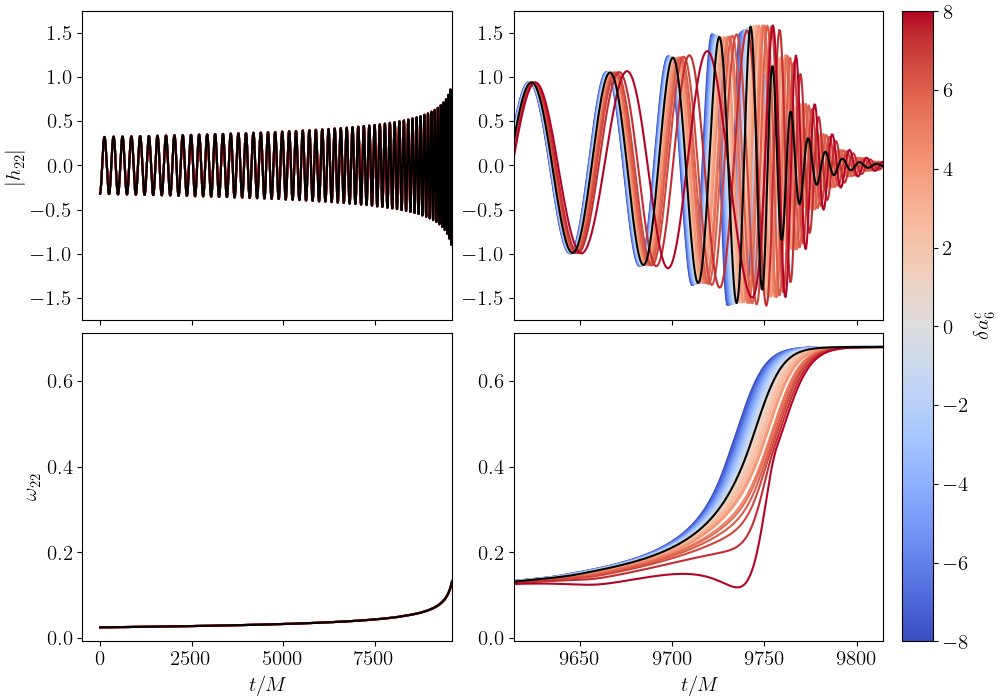
\includegraphics[width=0.49\textwidth]{figs/delta_a6c_-8.0_8.0.png}
    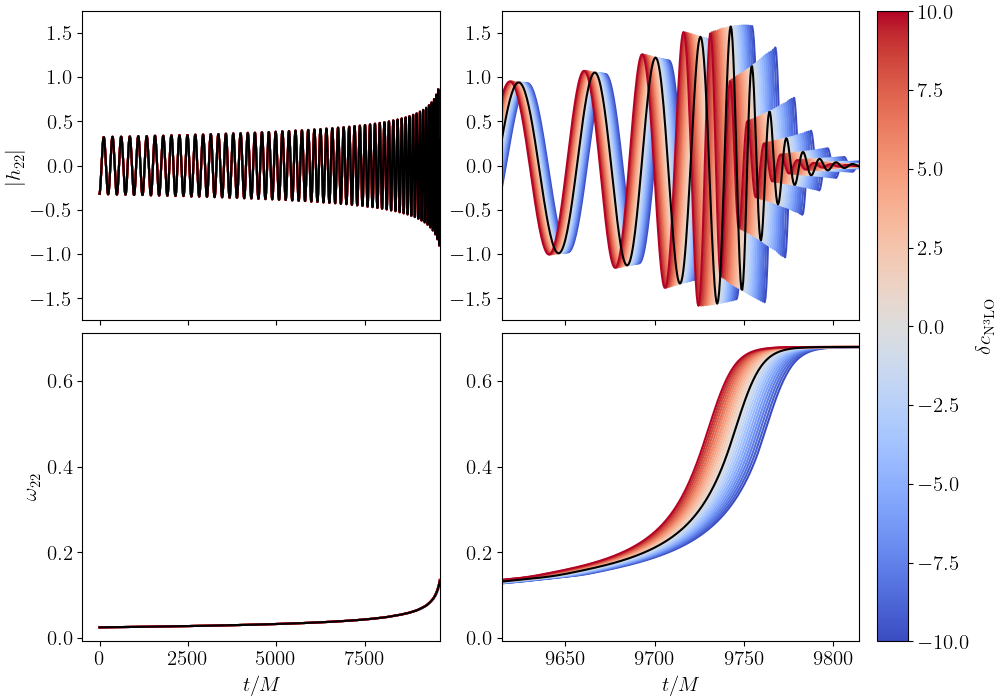
\includegraphics[width=0.49\textwidth]{figs/delta_cN3LO_-10.0_10.0.png}
    \caption{\label{fig:a6c3}
    Effect of the variation of $a_6^{\rm c}$ and $\c3$ on the $(2,2)$ mode real part and frequency
    for a binary with $q = 1, \chi_1 = \chi_2 = 0.6$. Waveforms here are aligned so they always start at $t = 0$,
    to better appreciate the cumulative effect of the deformed dynamics. $\delta a_6^c$ and $\delta \c3$ cause a slightly
    delayed or accelerated late inspiral and plunge, shifting the phase of the signal. The model is quite
    sensitive to the increase of $a_6^c$, delivering unphysical results for deviations $\geq 8$ in this case.
    This is partly due to the failure of the \ac{nqc} corrections in enforcing a smooth transition to the ringdown
    portion of the waveform. Dynamically, a broader range of values is allowed for $\delta a_{6}^c$, but
    if the deviation is large enough the warped potential leads to unphysical late dynamics.
    We see that an increase in $a_6^c$ delays the merger, while a decrease moves it forward slightly. The
    opposite is true for $\c3$ in this case; with negative spins it would instead be the same (i.e.,
    an increase in $\c3$ would delay the merger in that case).}
\end{figure*}

\begin{figure*}
    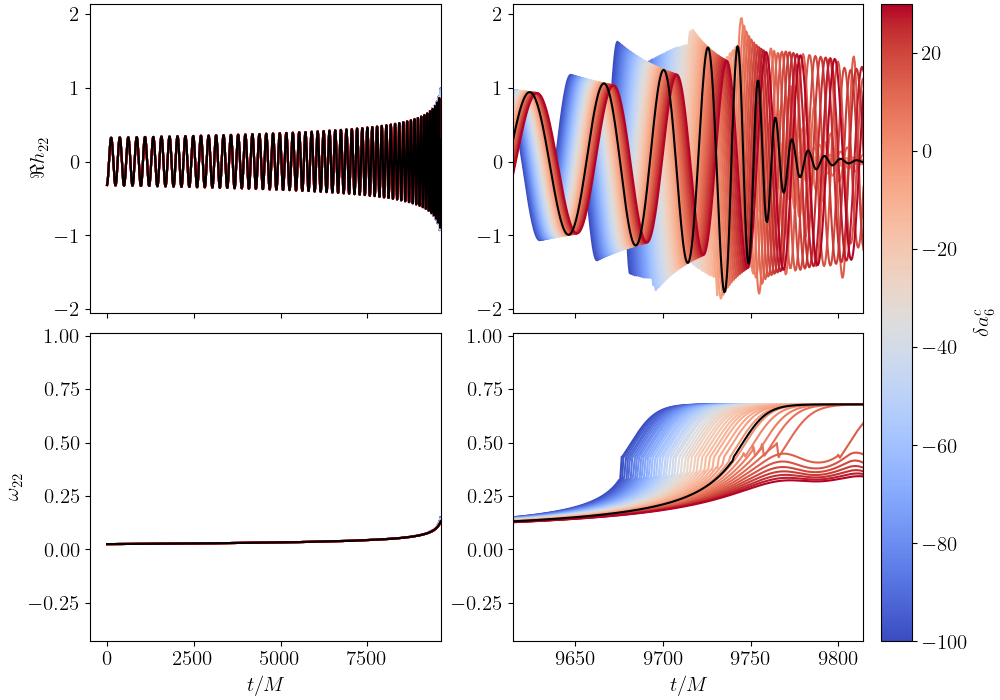
\includegraphics[width=0.49\textwidth]{figs/delta_a6c_-100.0_30.0.png}
    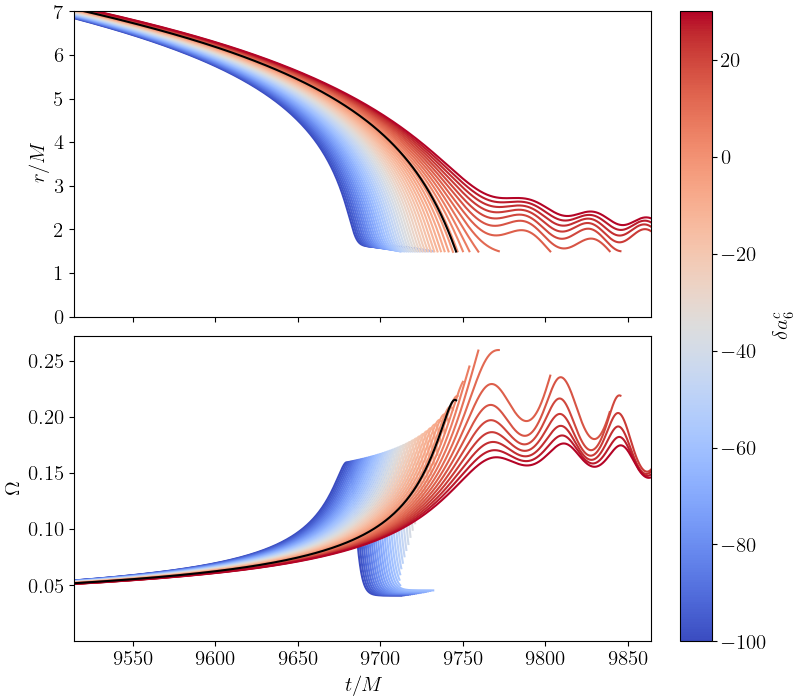
\includegraphics[width=0.49\textwidth]{figs/delta_a6c_-100.0_30.0_dyn.png}
    \caption{\label{fig:a6c3_nqc}
    Effect of the variation of $a_6^{\rm c}$ on the $(2,2)$ mode real part and frequency (left) and the
    orbital dynamics (right), for a binary with $q = 1, \chi_1 = \chi_2 = 0.6$. \ac{nqc} corrections are not
    applied here.
    Waveforms here are aligned so they always start at $t = 0$, to better appreciate the cumulative effect of the
    deformed dynamics. Compared to Fig.~\ref{fig:a6c3}, $a_6^c$ here takes values in a much larger interval,
    only leading to pathological results when the misshaped potential $A$ causes unphysical late dynamics.}
\end{figure*}

\begin{figure*}
    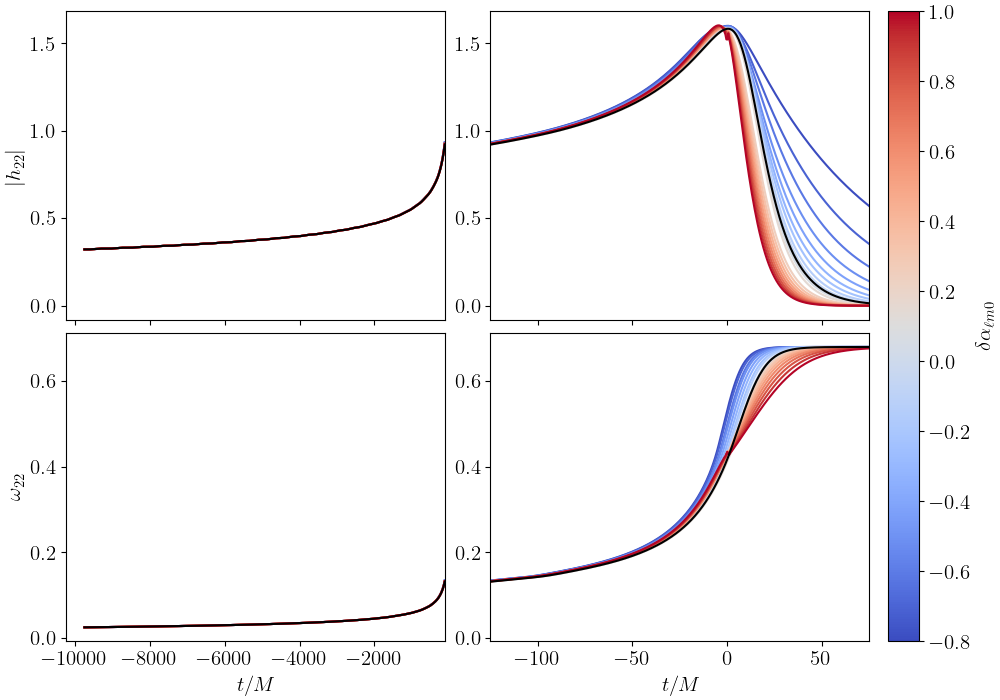
\includegraphics[width=0.49\textwidth]{figs/delta_alpha220_-0.8_1.0.png}
    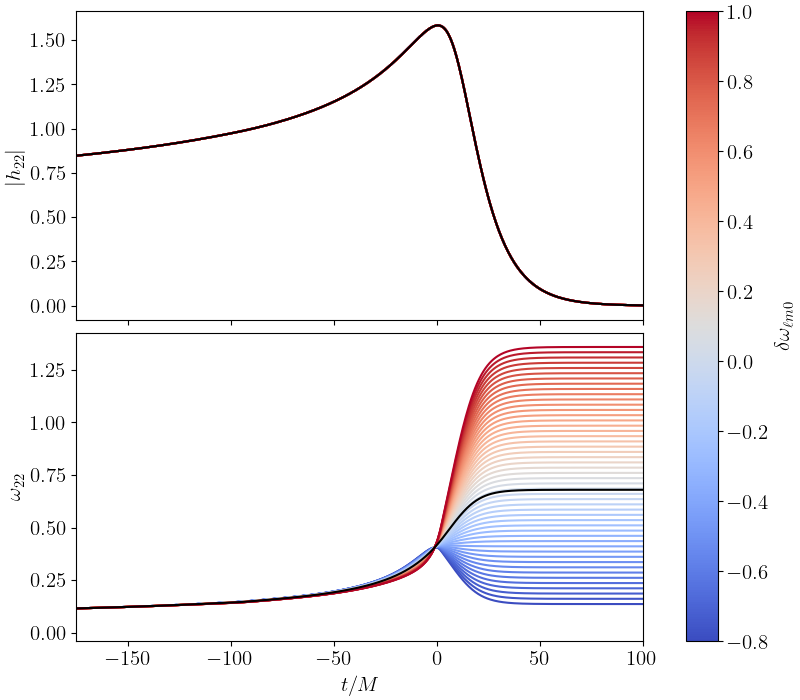
\includegraphics[width=0.49\textwidth]{figs/delta_omg220_-0.8_1.0.png}
    \caption{\label{fig:qnmdev}
    Effect of the variation of $\alpha_{220}$ and $\omega_{220}$ on the $(2,2)$ mode amplitude and frequency
    for a binary with $q = 1, \chi_1 = \chi_2 = 0.6$. Waveforms here are aligned so that for each
    $t = 0$ corresponds to the peak of $|h_{22}|$. An increase in the inverse damping time leads to a faster
    decaying ringdown, and vice-versa; this also affects the frequency evolution due to the structure of the
    ringdown model. Shifting the frequency does not instead significantly affect the amplitude.}
\end{figure*}

\begin{figure*}
    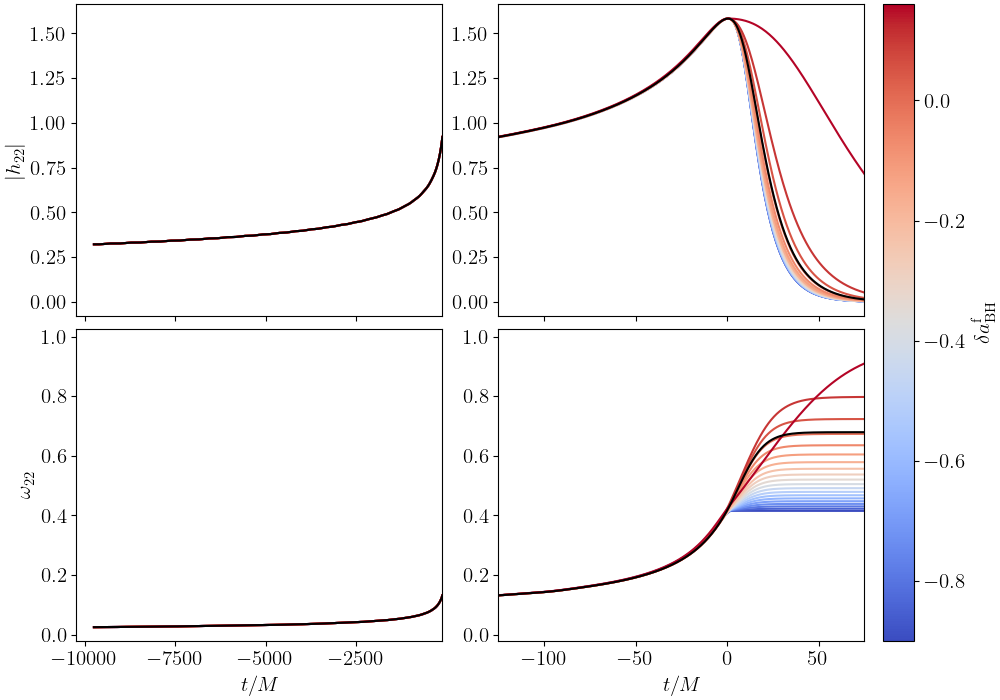
\includegraphics[width=0.49\textwidth]{figs/delta_abhf_-0.9_0.16.png}
    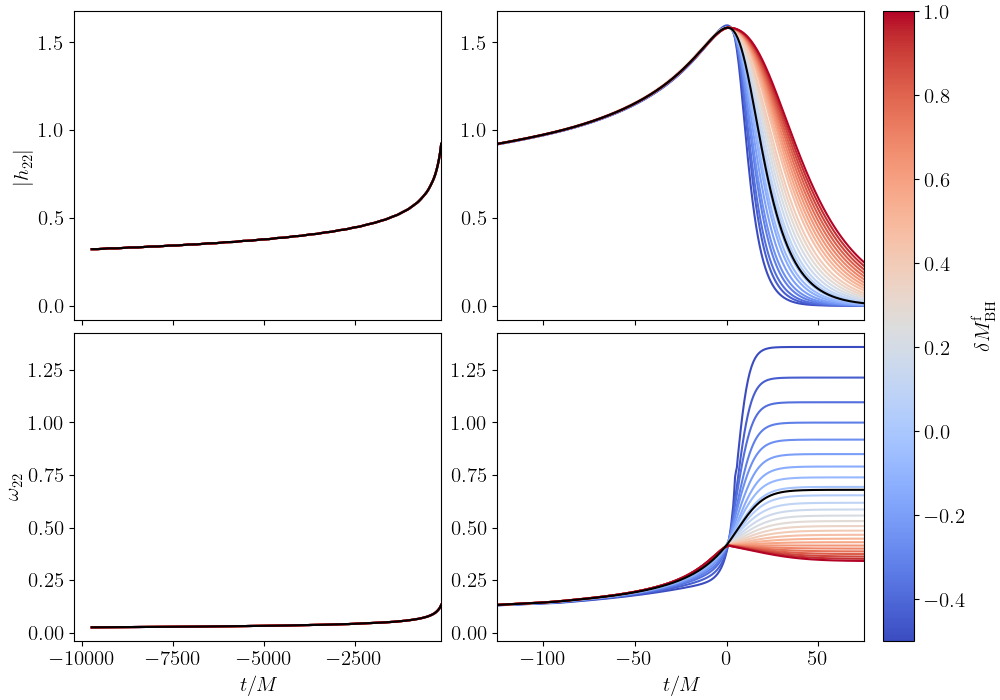
\includegraphics[width=0.49\textwidth]{figs/delta_Mbhf_-0.5_1.0.png}
    \caption{\label{fig:remnantdev}
    Effect of the variation of $\mbhf$ and $\abhf$ on the $(2,2)$ mode amplitude and frequency
    for a binary with $q = 1, \chi_1 = \chi_2 = 0.6$. Waveforms here are aligned so that for each
    $t = 0$ corresponds to the peak of $|h_{22}|$. An increase in the inverse damping time leads to a faster
    decaying ringdown, and vice-versa, as expected; this also affects the frequency evolution due to the structure of the
    ringdown model. Shifting the frequency does not instead significantly affect the amplitude.}
\end{figure*}

\begin{figure*}
    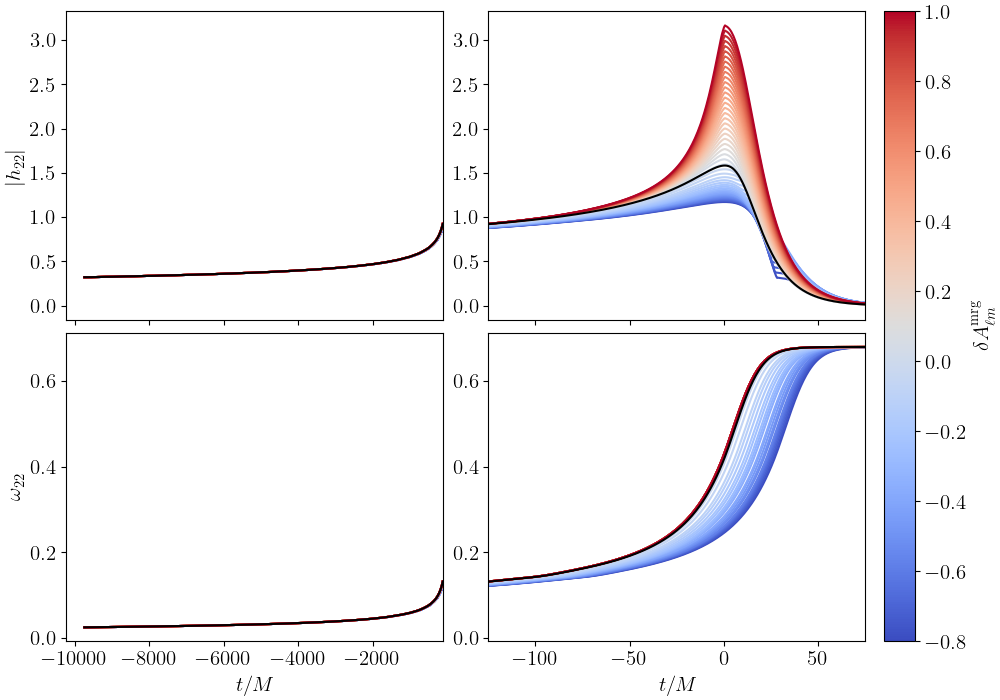
\includegraphics[width=0.49\textwidth]{figs/delta_A22_mrg_-0.8_1.0.png}
    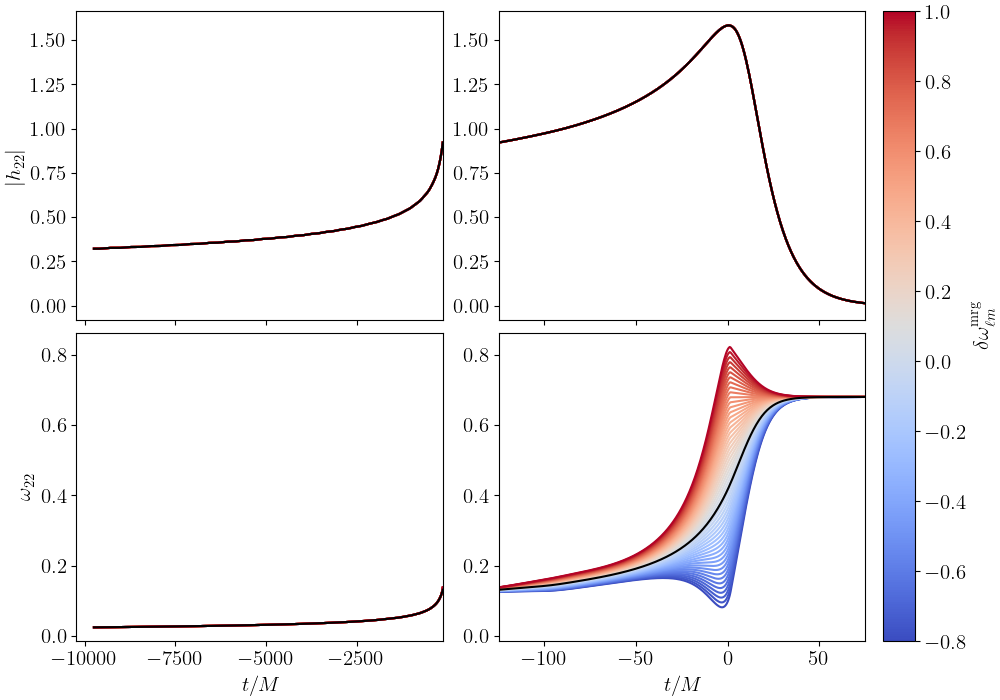
\includegraphics[width=0.49\textwidth]{figs/delta_Omg22_mrg_-0.8_1.0.png}
    \caption{\label{fig:mrgdev}
    Effect of the variation of $\amrg{22}$ and $\omgmrg{22}$ on the $(2,2)$ mode amplitude and frequency
    for a binary with $q = 1, \chi_1 = \chi_2 = 0.6$. Waveforms here are aligned so that for each
    $t = 0$ corresponds to the peak of $|h_{22}|$. Here we see how the shift in the merger quantities carries
    over to the NQC corrections, which enforce a match between the inspiral and ringdown. Increasing the amplitude
    does not change the location of the peak. Decreasing it however does (as is clear by the frequency plot),
    while also causing in the more extreme cases a non-smooth transition to the ringdown part of the signal.}
\end{figure*}

\begin{figure*}
    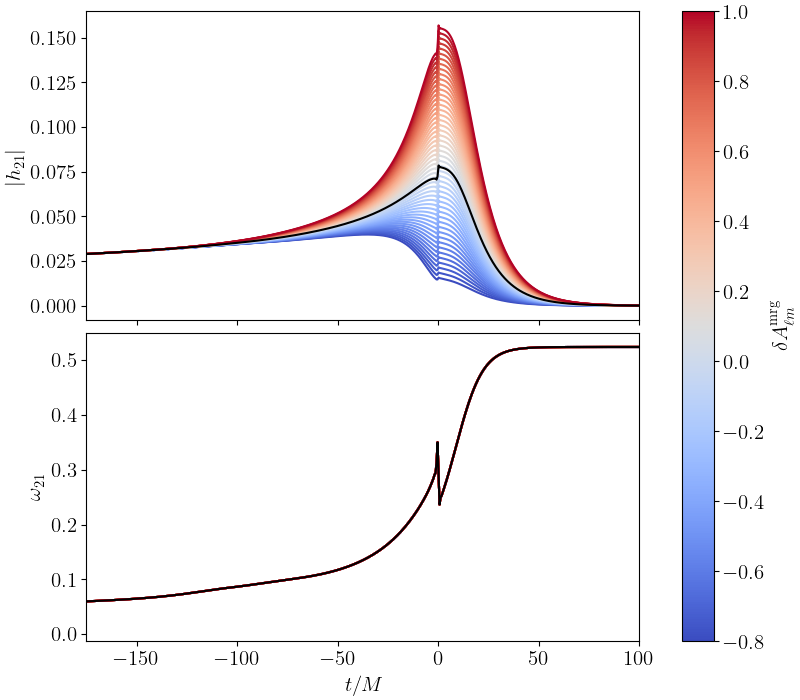
\includegraphics[width=0.49\textwidth]{figs/delta_A21_mrg_-0.8_1.0.png}
    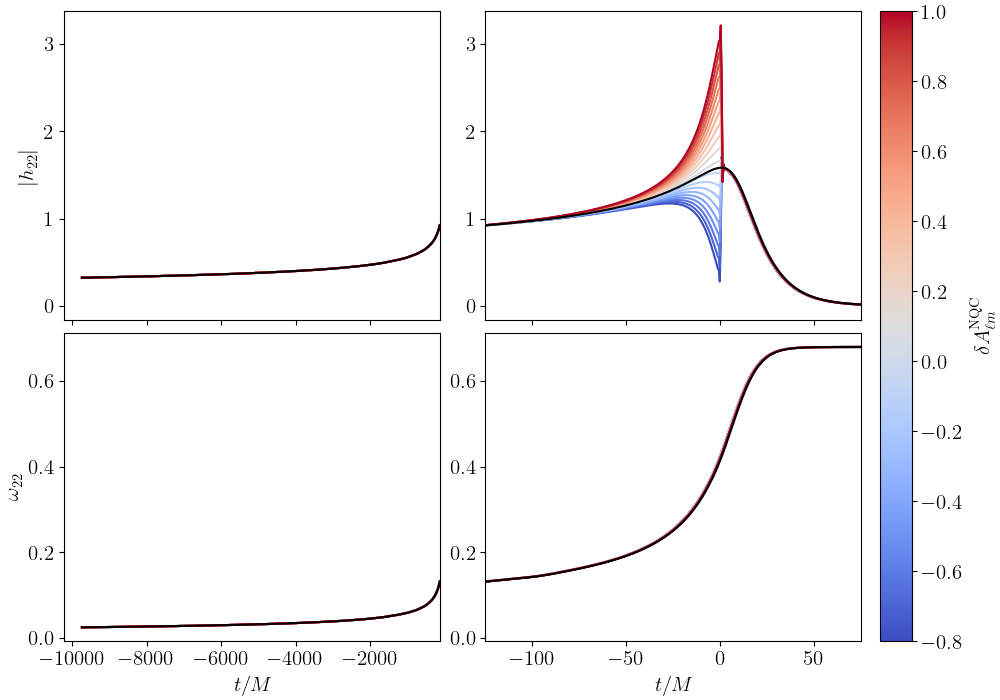
\includegraphics[width=0.49\textwidth]{figs/delta_A22_nqc_-0.8_1.0.png}
    \caption{\label{fig:bad_dev_mrgnqc}
    \textit{Left:} Effect of the variation of $\amrg{21}$ on the $(2,1)$ mode of the waveform
    for a binary with $q = 2, \chi_1 = \chi_2 = 0.6$.
    For this multipole, the NQC point quantities are computed from the post-merger model, instead of using
    dedicated fits as would be default in \dali. This way, the inspiral part of the waveform is
    consistently deformed as well so as to link up more smoothly with the ringdown (with varying outcomes).
    \textit{Right:} Variation of $\anqc{22}$ for a binary with $q = 1, \chi_1 = \chi_2 = 0.6$. The
    deformed NQC corrections here are not matched to a similarly modified post-merger signal, causing a discontinuity.}
\end{figure*}

\section{Application to data analysis}
\todo{Anyone who ran stuff, so Nic and Jake? }

\subsection{\ac{gw} \ac{pe}}
\todo{Quick recap of bayesian inference for GW}
\todo{Discuss settings for the \ac{pe} runs, e.g. sampler, priors, etc.}

\subsection{Model injections}
\RG{We may keep or nuke this section, depending on whether we want to. It is not strictly necessary,
but it does show that the model is sane (and we could potentially discuss degeneracies among the deviation parameters,
e.g. final mass and spin vs damping time etc)}

\subsection{\ac{nr} injections}

\subsection{Real data}

\section{Conclusion}
\todo{all}

\bibliography{refs, local}

\end{document}
